\documentclass[pdf]{beamer}
\mode<presentation>{}
\usetheme{Dresden}
\usepackage{apalike}
\usepackage{graphicx}
\usepackage{subcaption}
\usepackage{pgfplotstable}
\usepackage{graphicx,psfrag}
\usepackage{mwe,tikz}\usepackage[percent]{overpic}
%% preamble
\title{Robust Computational Models for Water Waves}
\author{Jordan Pitt, Stephen Roberts and Christopher Zoppou \\ Australian National University}
\newcommand\solidrule[1][0.25cm]{\rule[0.5ex]{#1}{1pt}}
\newcommand\dashedrule{\mbox{\solidrule[2mm]\hspace{2mm}\solidrule[2mm]}}
\newcommand{\dotrule}[1]{%
	\parbox[]{#1}{\dotfill}}

\begin{document}
%% title frame
\section{Introduction}
\begin{frame}
\titlepage
\end{frame}
\begin{frame}{Outline of the Presentation}
	%Modelling Process
	%SWWE
	%Serre
	%My Work
	
%	\begin{itemize}
%		\item Water Wave Modelling
%		\item Robust Computational Models
%	\end{itemize}
\end{frame}

\section{Water Wave Modelling}
\begin{frame}{Modelling}
	%Picture Physical Process -> Mathematical Description -> Studying Mathematical Description (Numerical Solution)
	\begin{figure}
		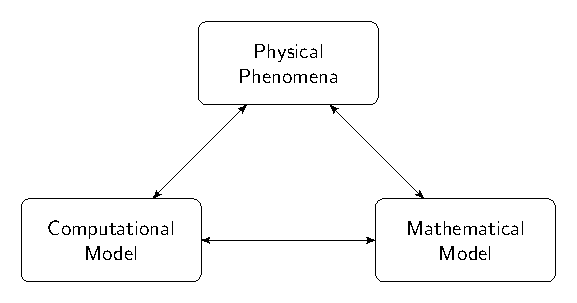
\includegraphics[width=\textwidth]{./Pics/ModelDiagrams/FlowChart.pdf}
	\end{figure}
\end{frame}
\begin{frame}{Physical Phenomena}
	%Picture Physical Process -> Mathematical Description -> Studying Mathematical Description (Numerical Solution)
	\begin{figure}
		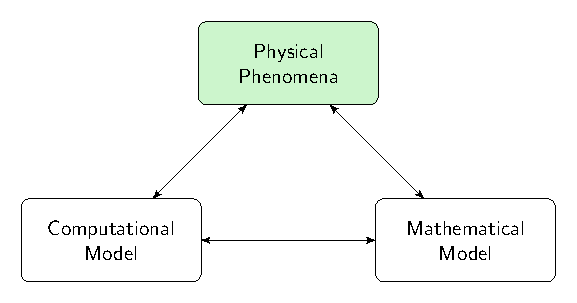
\includegraphics[width=\textwidth]{./Pics/ModelDiagrams/FlowChartHigh1G.pdf}
	\end{figure}
\end{frame}
\begin{frame}{Physical Phenomena: Water Waves}
	Water wave hazards:
		\begin{itemize}
			\item Tsunamis
			\item Storm Surges
			\item Rogue Waves
		\end{itemize}
	\smallskip
	Phenomena caused by water waves:
		\begin{itemize}
			\item Nutrient Transport
			\item Beach Erosion
			\item Breakup of Sea Ice
		\end{itemize}
\end{frame}
%Cool pictures
\begin{frame}{Typical Scenario}
	\begin{figure}
		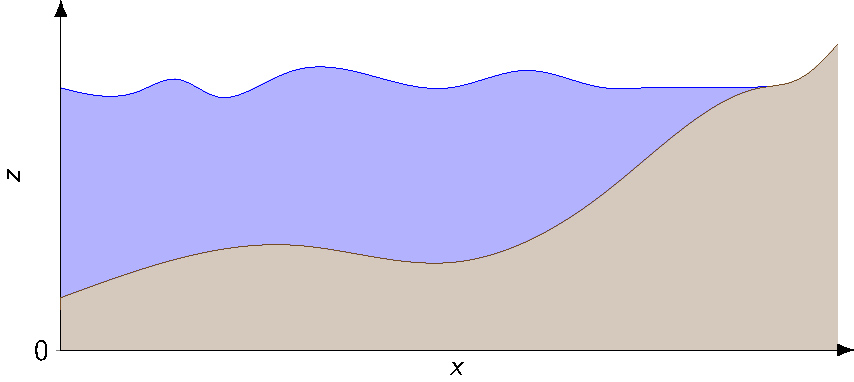
\includegraphics[width=\textwidth]{./Pics/WaterModelDiagrams/FressSurface.pdf}
	\end{figure}
\end{frame}


\subsection{Free Surface Flows}
\begin{frame}{Mathematical Model}
	%Picture Physical Process -> Mathematical Description -> Studying Mathematical Description (Numerical Solution)
	\begin{figure}
		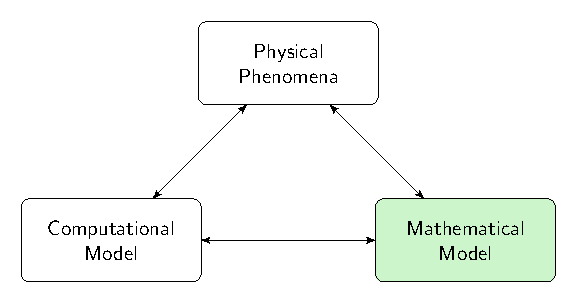
\includegraphics[width=\textwidth]{./Pics/ModelDiagrams/FlowChartHigh2G.pdf}
	\end{figure}
\end{frame}
\begin{frame}{Full Water Model}
	\begin{figure}
		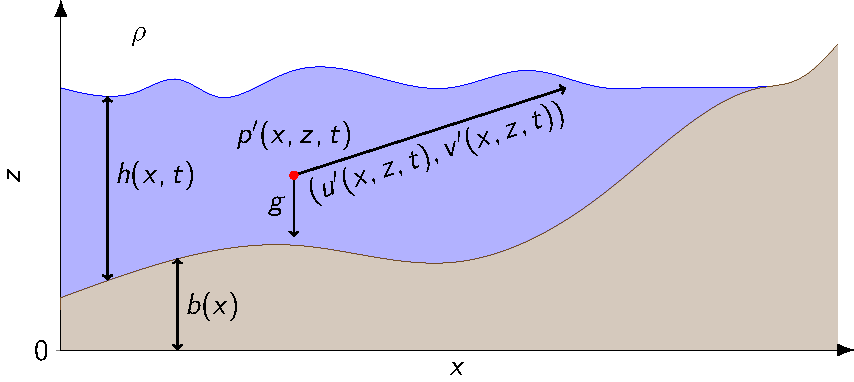
\includegraphics[width=\textwidth]{./Pics/WaterModelDiagrams/NavierStokes.pdf}
	\end{figure}
\end{frame}
\begin{frame}{Pros and Cons}
	Pro:
	\begin{itemize}
		\item Models all water behaviour very well 
	\end{itemize}
	Con:
	\begin{itemize}
		\item Complex mainly due to number of terms $u$, $v$, $p$, $h$ and $b$. 
		\item No efficient computational models at the scale necessary for natural disasters
	\end{itemize}
	Require a simpler mathematical model
\end{frame}


\subsection{Shallow Water Wave Model}
\begin{frame}{Shallow Water Wave Model}
	\begin{figure}
		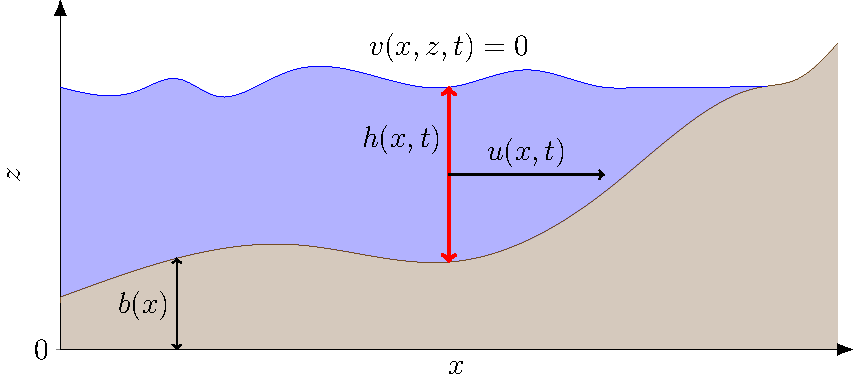
\includegraphics[width=\textwidth]{./Pics/WaterModelDiagrams/SWWE.pdf}
	\end{figure}
\end{frame}
\begin{frame}{Assumptions}
	\begin{itemize}
		\item $u(x,z,t)$ constant in $z$
		\item $v(x,z,t) = 0$
		\item $p(x,z,t) = g\left[ \left(h(x,t) - b(x)\right) - z\right]$
	\end{itemize}
\end{frame}
\begin{frame}{Equations}
	\begin{align}
	&\frac{\partial h}{\partial t} + \frac{\partial }{\partial x}\left( uh\right) = 0 \\ \nonumber \\
	&\frac{\partial u h}{\partial t} + \frac{\partial }{\partial x}\left( u^2h + \frac{1}{2}gh^2\right) + gh\frac{\partial b}{\partial x} = 0
	\end{align}
\end{frame}
\begin{frame}{Pros and Cons}
	Pro:
	\begin{itemize}
		\item Far simpler than the full water wave model
		\item Models waves with long wavelengths very well 
		\item Shows good agreement with experimental results
	\end{itemize}
	Cons:
	\begin{itemize}
		\item No dispersion
		\item Poor model for short waves 
	\end{itemize}
\end{frame}
\begin{frame}{Computational Model}
		\begin{figure}
			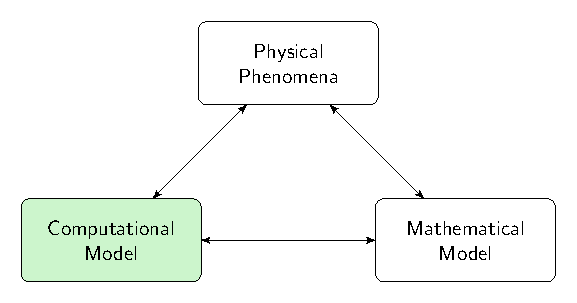
\includegraphics[width=\textwidth]{./Pics/ModelDiagrams/FlowChartHigh3G.pdf}
		\end{figure}
\end{frame}

\begin{frame}{ANUGA}
	\begin{itemize}
		\item 1999 : Stephen Roberts and Chris Zoppou Paper solving SWWE with a Finite Volume Method
		\item 2004 : ANUGA development begins originally focusing on storm surges
		\item 2005 : ANUGA refocused to tsunamis
		\item 2006 : ANUGA has first public release
	\end{itemize}
\end{frame}


\begin{frame}{Pros and Cons}
	Pros
	\begin{itemize}
	\item Efficient, robust and accurate computational model based on the SWWE
	\end{itemize}
	Cons
	\begin{itemize}
	\item No dispersion because of the SWWE
	\item SWWE not valid for shorter wavelengths
	\item Recent papers suggest dispersion maybe important for modelling tsunamis
	\end{itemize}
\end{frame}

\begin{frame}{Outcome}
 New Project at the ANU to build computational models from dispersive mathematical models
\end{frame}
%mention previous work of ANU


\subsection{Serre Model}
\begin{frame}{Mathematical Model}
	%Picture Physical Process -> Mathematical Description -> Studying Mathematical Description (Numerical Solution)
	\begin{figure}
		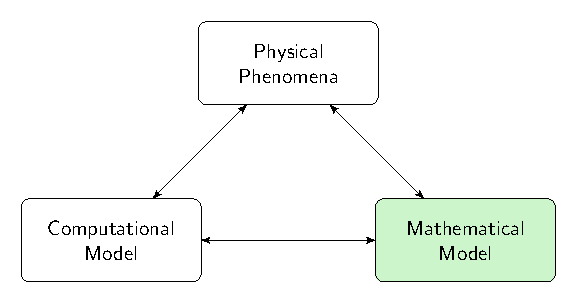
\includegraphics[width=\textwidth]{./Pics/ModelDiagrams/FlowChartHigh2G.pdf}
	\end{figure}
\end{frame}
\begin{frame}{Serre Model}
	\begin{figure}
		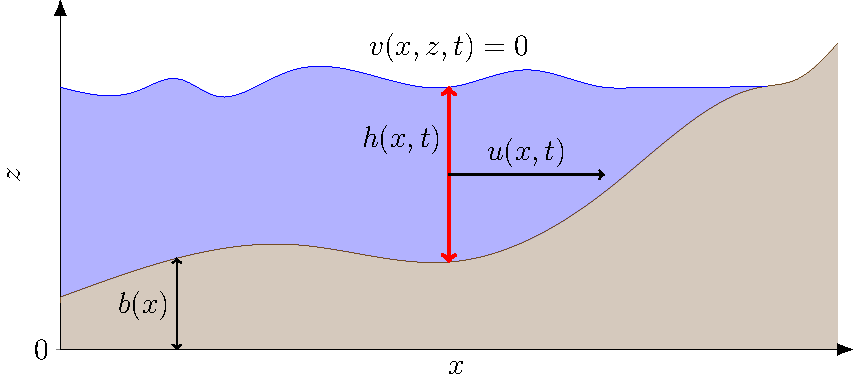
\includegraphics[width=\textwidth]{./Pics/WaterModelDiagrams/SWWE.pdf}
	\end{figure}
\end{frame}
\begin{frame}{Assumptions}
	\begin{itemize}
		\item $u(x,z,t)$ constant in $z$
		\item $v(x,z,t) = u\frac{\partial b}{\partial x} - (z - b)\frac{\partial b}{\partial x}$
		\item $p(x,z,t) = g\xi  + \xi { \color{red}\Psi } + \frac{1}{2} \xi \left(2h - \xi\right) { \color{blue} \Phi }$
	\end{itemize}
		with
		\begin{align*}
		&{ \color{red}\Psi }  = \dfrac{\partial b}{\partial x}\left(\dfrac{\partial u}{\partial t} + u\dfrac{\partial u}{\partial x} \right)  + u^2\dfrac{\partial^2 b}{\partial x^2}, \\&
		{ \color{blue} \Phi }  = \dfrac{\partial u }{\partial x} \dfrac{\partial u}{\partial x} -u \dfrac{\partial^2 u}{\partial x^2}  - \dfrac{\partial^2 u}{\partial x \partial t} .
		\end{align*}
\end{frame}
\begin{frame}{Equations}
	\begin{subequations}
		\begin{align*}
		&\frac{\partial h}{\partial t} + \dfrac{\partial (uh)}{\partial x} = 0,  \\ \\
		&\dfrac{\partial (uh)}{\partial t} + \dfrac{\partial}{\partial x} \left ( u^2h + \dfrac{gh^2}{2} + \dfrac{h^2}{2}{ \color{red}\Psi } + \dfrac{h^3}{3}{ { \color{blue} \Phi } }  \right )  +  \dfrac{\partial b}{\partial x} \left (gh +   h { \color{red}\Psi } + \dfrac{h^2}{2}{ { \color{blue} \Phi } }  \right ) = 0
		\end{align*}
	\end{subequations}
\end{frame}
\begin{frame}{Pros and Cons}
	Pro:
	\begin{itemize}
		\item Far simpler than the Euler equations
		\item Includes dispersive effects
		\item Still a good model for long wavelength waves and also a good model for shorter wavelengths
		\item Considered one of the best models for water waves up to wave breaking
	\end{itemize}
	Cons:
	\begin{itemize}
		\item More complicated than the SWWE due to extra terms
		\item No well developed, efficient robust computational models for three dimensional flows over complex geometries. 
	\end{itemize}
\end{frame}
\begin{frame}{Computational Model}
	%Picture Physical Process -> Mathematical Description -> Studying Mathematical Description (Numerical Solution)
	\begin{figure}
		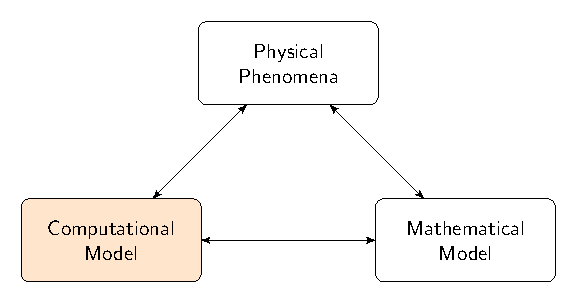
\includegraphics[width=\textwidth]{./Pics/ModelDiagrams/FlowChartHigh3O.pdf}
	\end{figure}
\end{frame}
\begin{frame}{Previous Work}
	\begin{itemize}
		\item 2014: Chris Zoppou's PhD thesis \\
			Demonstrated computational model based on Finite Volume Method for the Serre equations with varying bathymetry in 1D.
		\item 2014: My Honours thesis \\
			Independent reproduction of Chris's work
	\end{itemize}
	Open problems:
	\begin{itemize}
		\item Model validation for steep gradients in the flow
		\item Solution in the presence of dry beds
		\item Extension to 3D flows
	\end{itemize}	
\end{frame}



\section{Robust Computational Model}
%Goal of thesis to develop numerical method that can handle dry beds and steep gradients using FEM and FVM

\begin{frame}{Thesis Goals}
	Solve these open problems:
	\begin{itemize}
		\item Are solutions in the presence of steep gradient correct?
		\item Solution in the presence of dry beds
		\item Extension to 3D flows
	\end{itemize}
	Technique: Develop a numerical method for the 2D Serre equations with a Finite Volume method at its core that can readily be extended to 3D flows and is well validated for dry beds and steep gradients. 
\end{frame}

\subsection{Method}


\subsection{ Model Validation for Steep Gradients in the Flow}
\begin{frame}{Statement of Problem}
	How do these initial conditions evolve?
	\begin{figure}
		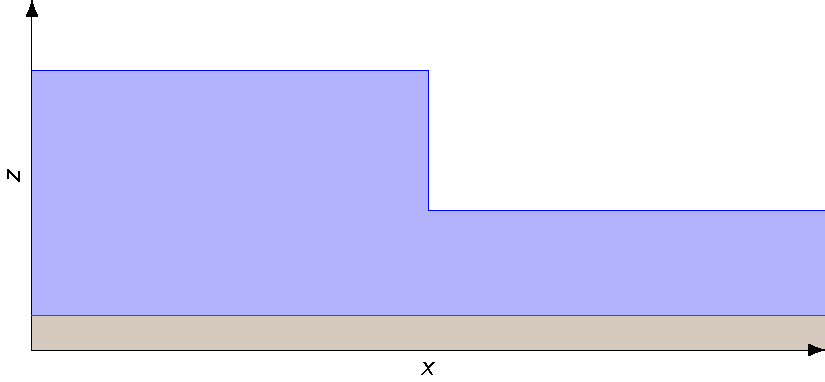
\includegraphics[width=\textwidth]{./Pics/SteepGradients/Wavetank.pdf}
	\end{figure}
\end{frame}	

%What was known
%Previous Work
%Improvements
\begin{frame}{What was known}
	\begin{itemize}
		\item No analytic solutions
		\item Asymptotic results for step gradient problems as $t \rightarrow \infty$
		\item Some experimental and numerical results comparisons (Chris's Thesis)
		\item A variety of numerical solutions some solving actual steep gradient problems and some  smoothing them
	\end{itemize}
\end{frame}

\begin{frame}{Solution}
	\begin{itemize}
		\item Demonstrated convergence to one solution for many numerical methods
		\item Investigated the effect of smoothing

	\end{itemize}
\end{frame}


\subsection{Solution in the Presence of Dry Beds}
%What was known
%Previous Work
%Improvements
\begin{frame}
\end{frame}

\end{document}